% !TEX root =  master.tex
\chapter{Optimierung und Potenziale}
\section{Optimierung der Poolgröße}
Im vorherigen Kapitel wurde aufgezeigt, dass die Effizienz einer Poolingmethode von zwei Parametern abhängt.
In Kombination ergeben diese beiden Werte die Wahrscheinlichkeit, mit welcher infizierte Personen innerhalb der Testgruppe sind.
\begin{itemize}
	\item \textbf{Prävalenz} Hieraus ergibt sich die Wahrscheinlichkeit, mit der Personen infiziert sind.
	Bei einem realen Testverfahren ist die Prävalenz ein externer Faktor.
	Sie ist Abhängig von der aktuellen Inzidenz und dem Umfeld der Testung.
	\item \textbf{Größe der Testgruppe} Diese kann vom Labor frei gewählt werden.
\end{itemize}

Dieser Zusammenhang ergibt die Funktion für den Erwartungswert:\newline
$\frac{Personenzahl}{(1 - (1-Prävalenz)^{Personenzahl} \cdot (Personenzahl + 1)) + ((1-Prävalenz)^{Personenzahl}) \cdot 1)}$

Für jede gegebene Prävalenz, lassen sich durch Auswahl der Personenanzahl unterschiedliche Verläufe der Effizienzkurve erreichen.
Die Anzahl der Personen pro Pool sollte deshalb anhand der Prävalenz gewählt werden, um den Erwartungswert zu maximieren.

Der Erwartungswert(Personenzahl, Prävalenz) lässt sich auch als Graph darstellen.
\begin{wrapfigure}{r}{0.48\textwidth}
	%\centering
	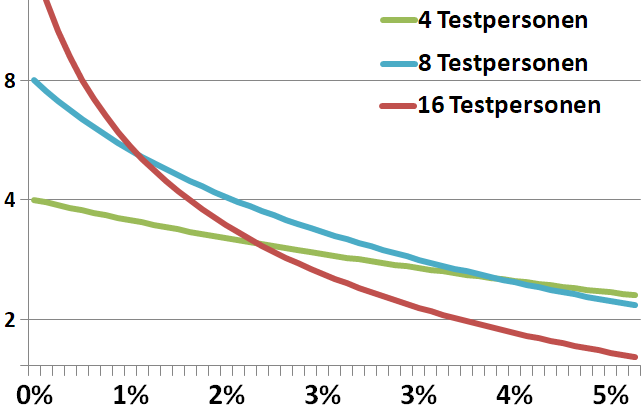
\includegraphics[width=.48\textwidth]{img/PraevalenzZuTestgruppe}
	\caption{\mbox{Effizienz unterschiedlicher} \mbox{Poolgrößen} nach Prävalenz\footnotemark}
\end{wrapfigure}
\footnotetext{Eigene Darstellung}
Wenn man eine der Variablen als Rahmenbedingung festsetzt, lässt sich der andere Wert gemeinsam mit der Effizienz als Diagramm zeichnen.
in Abbildung X.X wird die Personenanzahl auf 4, 8 und 16 festgesetzt und der Erwartungswert in Abhängigkeit der Prävalenz dargestellt.
Zu erkennen ist, dass höhere Personenzahlen bei niedrigen Prävalenzen die Effizienz enorm steigern können.
Wenn die Prävalenz allerdings steigt, werden die großen Pools schnell anfällig für Nachtestungen und verlieren so überproportional an Effizienz.

\cleardoublepage

Alternativ zur Darstellung nach Poolgröße kann auch die Prävalenz als gegeben festgesetzt werden.
In Abbildung X.X wird hierfür jedes Prävalenzniveau als eigener Graph dargestellt.
Das Optimum für die aktuelle Prävalenz liegt hierbei immer am Hochpunkt.
Die Poolgröße und hieraus resultierende Effizienz kann direkt auf den Achsen abgelesen werden.
\begin{figure}[h]
	\centering
	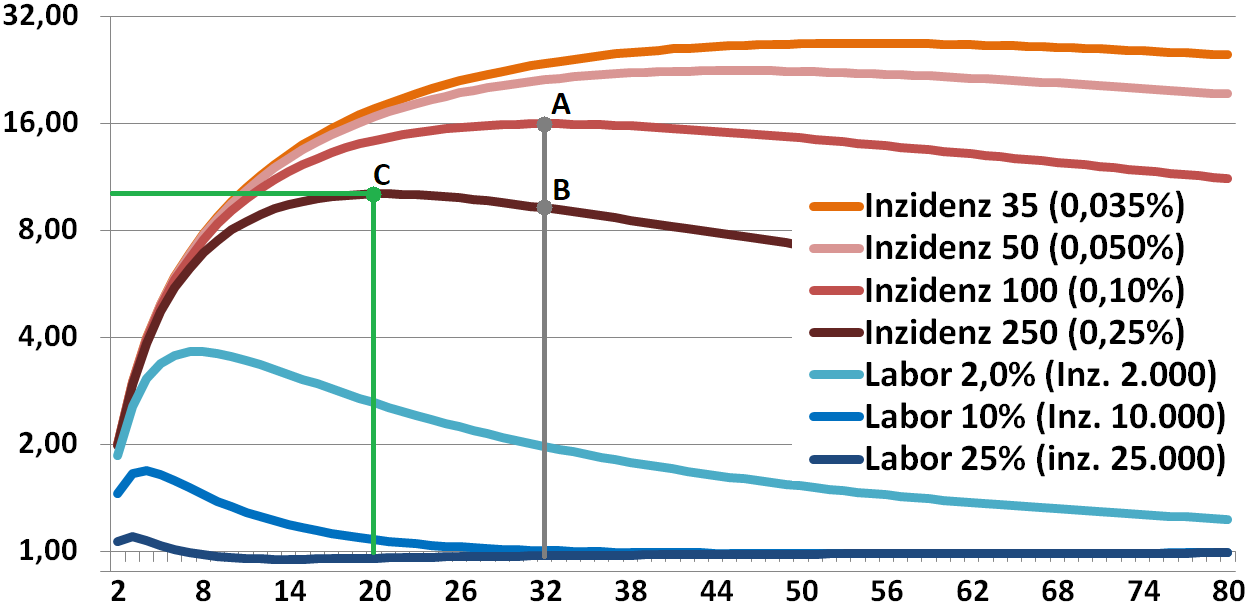
\includegraphics[width=1\textwidth]{img/EffizienzTestgruppePfeile}
	\caption{Effizienz eines Pools mit drei Personen nach Prävalenz\footnotemark}
\end{figure}
\footnotetext{Eigene Darstellung}

\begin{wraptable}{r}{7.7cm}
	\begin{tabular}{|r|r|c|r|}
		\hline
		Inzidenz&Prävalenz&Personen&Effizienz\\
		\hline
		35 & 0,00035 & 54 & 26,9x\\
		\hline
		50 & 0,00050 & 45 & 22,5x \\
		\hline
		100 & 0,00100 & 32 & 15,9x \\
		\hline
		250 & 0,00250 & 21 & 10,1x \\
		\hline
		2.000 & 0,02 & 8 & 3,6x\\
		\hline
		10.000 & 0,10  & 4 & 1,7x\\
		\hline
		25.000 & 0,25 & 3 & 1,1x\\
		\hline
	\end{tabular}
	\caption{Effizienzsteigerungspotenzial\footnotemark}
\end{wraptable} 
\footnotetext{Eigene Darstellung, Eine vollständige Gegenüberstellung in tabellarischer Form ist im Anhang dargestellt.}
Die bisherige Inzidenz lag bei 100.
Das Pooling an Punkt A war mit 32 Personen effizient und erreichte einen Faktor von 15,93.
Wenn die Inzidenz sich auf 250 erhöht, sinkt die Effizienz bei unveränderten Poolgröße auf Punkt B. Die Effizienz ist nur noch 9,24.
Für das neue Inzidenzniveau bei 250 kann das Pooling optimiert werden, indem die Poolgröße auf 20 gesenkt wird.
Dies bewirkt eine Linksverschiebung entlang der 250-Linie zu Punkt C.
Hier kann eine Effizienz von 10,12x erwartet werden.

\cleardoublepage

\section{Ausblick: Komplexe Poolingverfahren}
Dieser Abschnitt widmet sich einem Ausblick auf komplexere Poolingverfahren, welche im Umfang dieser Arbeit nicht näher beleuchtet werden können.
Durch die zunehmende Komplexität ergeben sich Potenziale für weitere Effizienzsteigerungen.
Diese sind allerdings auch mit neuen Risiken verbunden.

\textbf{Mehrdimensionale Pools}\ haben das Ziel, durch Überlappung der Pools den Bedarf einer Nachtestung bei einzelnen Positivfällen zu minimieren.
Die Testpersonen werden in einer AxB-Matrix angeordnet.
Die Proben werden dann für jede Spalte und jede Reihe gepoolt.
Allgemein formuliert lässt sich sagen:
Testbedarf pro Person =
$\frac{A+B}{A\cdot B}$

\begin{wrapfigure}{r}{0.48\textwidth}
	%\centering
	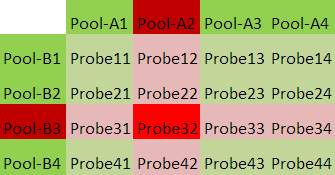
\includegraphics[width=.48\textwidth]{img/2d_Pool_1Positiv}
	\caption{Zweidimensionaler Pool mit einer positiven Probe\footnotemark}
\end{wrapfigure}
\footnotetext{Eigene Darstellung}
Für eine Testgruppe von 25 Personen, welche in einer 5x5 Matrix angeordnet sind, werden somit 5+5 Tests benötigt.
Die Effizienz läge bei 2,5x wenn alle Personen negativ getestet werden.
Vergleichen mit dem eindimensionalen Poolingverfahren klingt das zunächst nicht nach sehr viel.
Allerdings ist dieses Verfahren robust gegen einzelne Positivfälle.
Dies kann bei hohen Prävalenzen einen Vorteil bietet, da nicht alle Testpersonen erneut getestet werden müssen.
Zwei Positivfälle lassen sich beispielsweise mit nur vier Nachtestungen auflösen.
Hieraus ergibt sich, dass 25 Personen mit 10+4 Tests aufgelöst wurden.
Das Verfahren behält also selbst bei zwei positiven Proben eine Effizienz von 1,79 und verspricht damit deutlich robuster gegen hohe Prävalenzen zu sein.

Viehweger beschreibt ein Verfahren, um bei einer Prävalenz von 2 Prozent noch eine Effizienzsteigerung um den Faktor 5x zu erreichen.\footnote{Viehweger Z14}
Das in dieser Arbeit beschriebene Verfahren kommt hier nur auf einen Erwartungswert von 3,6x.
Für die Überprüfung von Verdachtsfällen mit hohen Prävalenzen, sollte deshalb diese Verfahren geprüft werden.

\cleardoublepage